% F049: native TikZ/PGFPlots, computed from the stated mathematical model.
\begin{center}
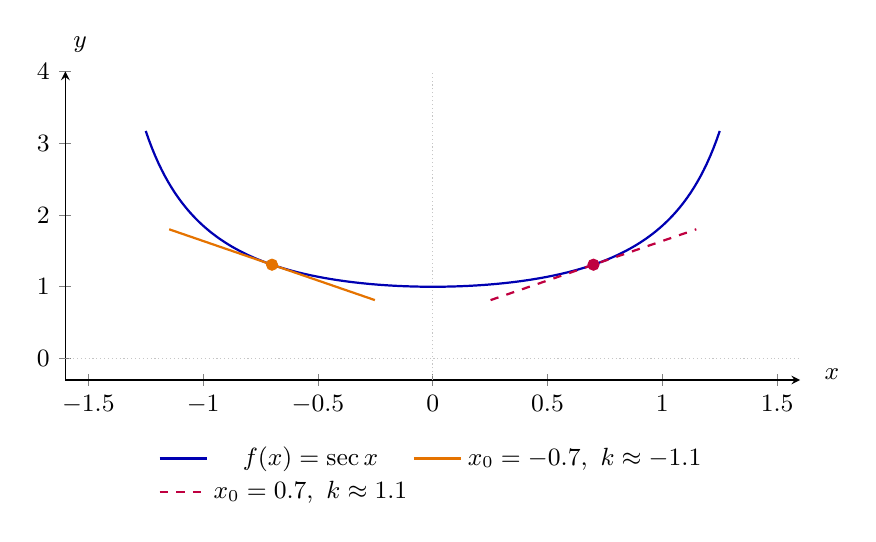
\begin{tikzpicture}[font=\small,>=stealth]
\begin{axis}[width=.90\linewidth,height=5.5cm,xmin=-1.6,xmax=1.6,ymin=-0.3,ymax=4,
axis lines=left,xlabel={$x$},ylabel={$y$},font=\small,
xlabel style={at={(axis description cs:1.02,.02)},anchor=west},
ylabel style={rotate=-90,at={(axis description cs:.02,1.03)},anchor=south},
legend style={at={(axis description cs:.5,-.18)},anchor=north,draw=none,fill=none,font=\small,legend columns=2},
unbounded coords=jump,clip=true,]
\addplot[gray!45,thin,densely dotted,forget plot] coordinates {(-1.6,0) (1.6,0)};
\addplot[gray!45,thin,densely dotted,forget plot] coordinates {(0,-0.3) (0,4)};
\addplot[blue!70!black,thick] coordinates {(-1.25,3.1713577) (-1.2361111,3.0444007) (-1.2222222,2.9277603) (-1.2083333,2.8202518) (-1.1944444,2.7208654) (-1.1805556,2.6287351) (-1.1666667,2.5431142) (-1.1527778,2.4633551) (-1.1388889,2.3888935) (-1.125,2.3192358) (-1.1111111,2.2539477) (-1.0972222,2.1926461) (-1.0833333,2.1349917) (-1.0694444,2.0806827) (-1.0555556,2.0294498) (-1.0416667,1.9810524) (-1.0277778,1.9352741) (-1.0138889,1.8919204) (-1,1.8508157) (-0.98611111,1.8118013) (-0.97222222,1.7747329) (-0.95833333,1.7394798) (-0.94444444,1.7059226) (-0.93055556,1.6739524) (-0.91666667,1.6434697) (-0.90277778,1.6143831) (-0.88888889,1.5866089) (-0.875,1.56007) (-0.86111111,1.5346956) (-0.84722222,1.51042) (-0.83333333,1.4871829) (-0.81944444,1.4649282) (-0.80555556,1.4436042) (-0.79166667,1.4231626) (-0.77777778,1.4035588) (-0.76388889,1.3847512) (-0.75,1.3667011) (-0.73611111,1.3493725) (-0.72222222,1.3327317) (-0.70833333,1.3167472) (-0.69444444,1.3013897) (-0.68055556,1.2866316) (-0.66666667,1.2724471) (-0.65277778,1.2588122) (-0.63888889,1.2457042) (-0.625,1.2331017) (-0.61111111,1.2209848) (-0.59722222,1.2093348) (-0.58333333,1.1981339) (-0.56944444,1.1873655) (-0.55555556,1.177014) (-0.54166667,1.1670646) (-0.52777778,1.1575034) (-0.51388889,1.1483173) (-0.5,1.1394939) (-0.48611111,1.1310216) (-0.47222222,1.1228894) (-0.45833333,1.1150868) (-0.44444444,1.1076041) (-0.43055556,1.100432) (-0.41666667,1.0935618) (-0.40277778,1.0869852) (-0.38888889,1.0806945) (-0.375,1.0746822) (-0.36111111,1.0689416) (-0.34722222,1.063466) (-0.33333333,1.0582493) (-0.31944444,1.0532857) (-0.30555556,1.0485698) (-0.29166667,1.0440964) (-0.27777778,1.0398608) (-0.26388889,1.0358584) (-0.25,1.032085) (-0.23611111,1.0285367) (-0.22222222,1.0252098) (-0.20833333,1.0221009) (-0.19444444,1.0192068) (-0.18055556,1.0165245) (-0.16666667,1.0140515) (-0.15277778,1.0117851) (-0.13888889,1.0097232) (-0.125,1.0078637) (-0.11111111,1.0062048) (-0.097222222,1.0047448) (-0.083333333,1.0034823) (-0.069444444,1.0024161) (-0.055555556,1.0015452) (-0.041666667,1.0008687) (-0.027777778,1.0003859) (-0.013888889,1.0000965) (0,1) (0.013888889,1.0000965) (0.027777778,1.0003859) (0.041666667,1.0008687) (0.055555556,1.0015452) (0.069444444,1.0024161) (0.083333333,1.0034823) (0.097222222,1.0047448) (0.11111111,1.0062048) (0.125,1.0078637) (0.13888889,1.0097232) (0.15277778,1.0117851) (0.16666667,1.0140515) (0.18055556,1.0165245) (0.19444444,1.0192068) (0.20833333,1.0221009) (0.22222222,1.0252098) (0.23611111,1.0285367) (0.25,1.032085) (0.26388889,1.0358584) (0.27777778,1.0398608) (0.29166667,1.0440964) (0.30555556,1.0485698) (0.31944444,1.0532857) (0.33333333,1.0582493) (0.34722222,1.063466) (0.36111111,1.0689416) (0.375,1.0746822) (0.38888889,1.0806945) (0.40277778,1.0869852) (0.41666667,1.0935618) (0.43055556,1.100432) (0.44444444,1.1076041) (0.45833333,1.1150868) (0.47222222,1.1228894) (0.48611111,1.1310216) (0.5,1.1394939) (0.51388889,1.1483173) (0.52777778,1.1575034) (0.54166667,1.1670646) (0.55555556,1.177014) (0.56944444,1.1873655) (0.58333333,1.1981339) (0.59722222,1.2093348) (0.61111111,1.2209848) (0.625,1.2331017) (0.63888889,1.2457042) (0.65277778,1.2588122) (0.66666667,1.2724471) (0.68055556,1.2866316) (0.69444444,1.3013897) (0.70833333,1.3167472) (0.72222222,1.3327317) (0.73611111,1.3493725) (0.75,1.3667011) (0.76388889,1.3847512) (0.77777778,1.4035588) (0.79166667,1.4231626) (0.80555556,1.4436042) (0.81944444,1.4649282) (0.83333333,1.4871829) (0.84722222,1.51042) (0.86111111,1.5346956) (0.875,1.56007) (0.88888889,1.5866089) (0.90277778,1.6143831) (0.91666667,1.6434697) (0.93055556,1.6739524) (0.94444444,1.7059226) (0.95833333,1.7394798) (0.97222222,1.7747329) (0.98611111,1.8118013) (1,1.8508157) (1.0138889,1.8919204) (1.0277778,1.9352741) (1.0416667,1.9810524) (1.0555556,2.0294498) (1.0694444,2.0806827) (1.0833333,2.1349917) (1.0972222,2.1926461) (1.1111111,2.2539477) (1.125,2.3192358) (1.1388889,2.3888935) (1.1527778,2.4633551) (1.1666667,2.5431142) (1.1805556,2.6287351) (1.1944444,2.7208654) (1.2083333,2.8202518) (1.2222222,2.9277603) (1.2361111,3.0444007) (1.25,3.1713577)};
\addlegendentry{$f(x)=\sec x$}
\addplot[orange!90!black,thick] coordinates {(-1.148,1.8008227) (-0.252,0.81409579)};
\addlegendentry{$x_0=-0.7,\ k\approx-1.1$}
\addplot[only marks,mark=*,orange!90!black,forget plot] coordinates {(-0.7,1.3074593)};
\addplot[purple,thick,dashed] coordinates {(0.252,0.81409579) (1.148,1.8008227)};
\addlegendentry{$x_0=0.7,\ k\approx1.1$}
\addplot[only marks,mark=*,purple,forget plot] coordinates {(0.7,1.3074593)};

\end{axis}
\end{tikzpicture}
\par\smallskip{\small $\cos x\ne0$；左右两侧切线斜率分别为负、正。}
\end{center}
